\documentclass[tikz,border=10pt]{standalone}
\usepackage{tikz}
\usetikzlibrary{angles, quotes, intersections}

\begin{document}
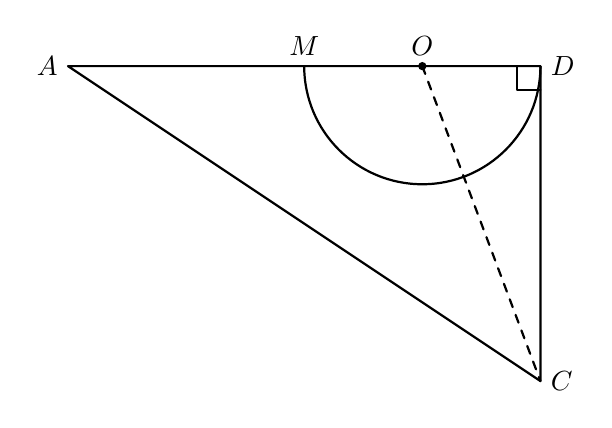
\begin{tikzpicture}[line cap=round, line join=round, >=stealth, thick]

    % 1. 定义关键点坐标 (可根据需要调整比例)
    \coordinate (D) at (0,0);
    \coordinate (A) at (-6,0);
    \coordinate (C) at (0,-4);
    \coordinate (O) at (-1.5,0); % 圆心 O 的位置
    \coordinate (M) at (-3,0);   % 点 M 的位置 (根据半径决定)

    % 2. 绘制直角三角形 ADC
    \draw (A) -- (D) -- (C) -- cycle;
    \draw [dashed] (O) -- (C);
    % 3. 绘制半圆弧 (以 O 为圆心，从 M 到 D，位于下方)
    % 半径为 |OD| = 1.5
    \draw (M) arc[start angle=180, end angle=360, radius=1.5];

    % 4. 绘制直角符号
    \draw (D) ++(-0.3,0) -- ++(0,-0.3) -- ++(0.3,0);

    % 5. 绘制圆心 O 的实心圆点
    \fill (O) circle (1.5pt);

    % 6. 标注文本
    % 使用 [above], [left] 等参数微调文字位置
    \node[left] at (A) {$A$};
    \node[above] at (M) {$M$};
    \node[above] at (O) {$O$};
    \node[right] at (D) {$D$};
    \node[right] at (C) {$C$};

\end{tikzpicture}
\end{document}